

%---------------------------------------------
\newpage % NOTE: The appendix title should be on its own page.
%---------------------------------------------
\chapter{Time-Lapse Movies}
\section{Early Season} 
\href{https://youtu.be/f_LF7-_opkc}{https://youtu.be/f\_LF7-\_opkc} 
\section{Mid Season} 
\href{https://youtu.be/J5fFBARJAu0}{https://youtu.be/J5fFBARJAu0}
\section{Late Season - Isothermal Development} 
\href{https://youtu.be/hLevt5xeN9o}{https://youtu.be/hLevt5xeN9o}

\chapter{BSTA Technical Details}
\section{Parts List}
\href{https://drive.google.com/file/d/1wrSelvj6EzlNViaM0zonwLIbumqkNpm5/view?usp=sharing}{https://drive.google.com/file/d/1wrSelvj6EzlNViaM0zonwLIbumqkNpm5/ \\ view?usp=sharing}
\section{CR1000 Code}
\href{https://drive.google.com/file/d/1Z6SDvXJ5vwWH153xJffSQQ8yu_DaKKHo/view?usp=sharing}{https://drive.google.com/file/d/1Z6SDvXJ5vwWH153xJffSQQ8yu_DaKKHo/ \\ view?usp=sharing}

\section{Design}
The following designs came from Charlie Luce and Tom Black with the USFS in Boise, ID during correspondence on October 18th, 2018. We used these diagrams to design and construct the BSTA. 
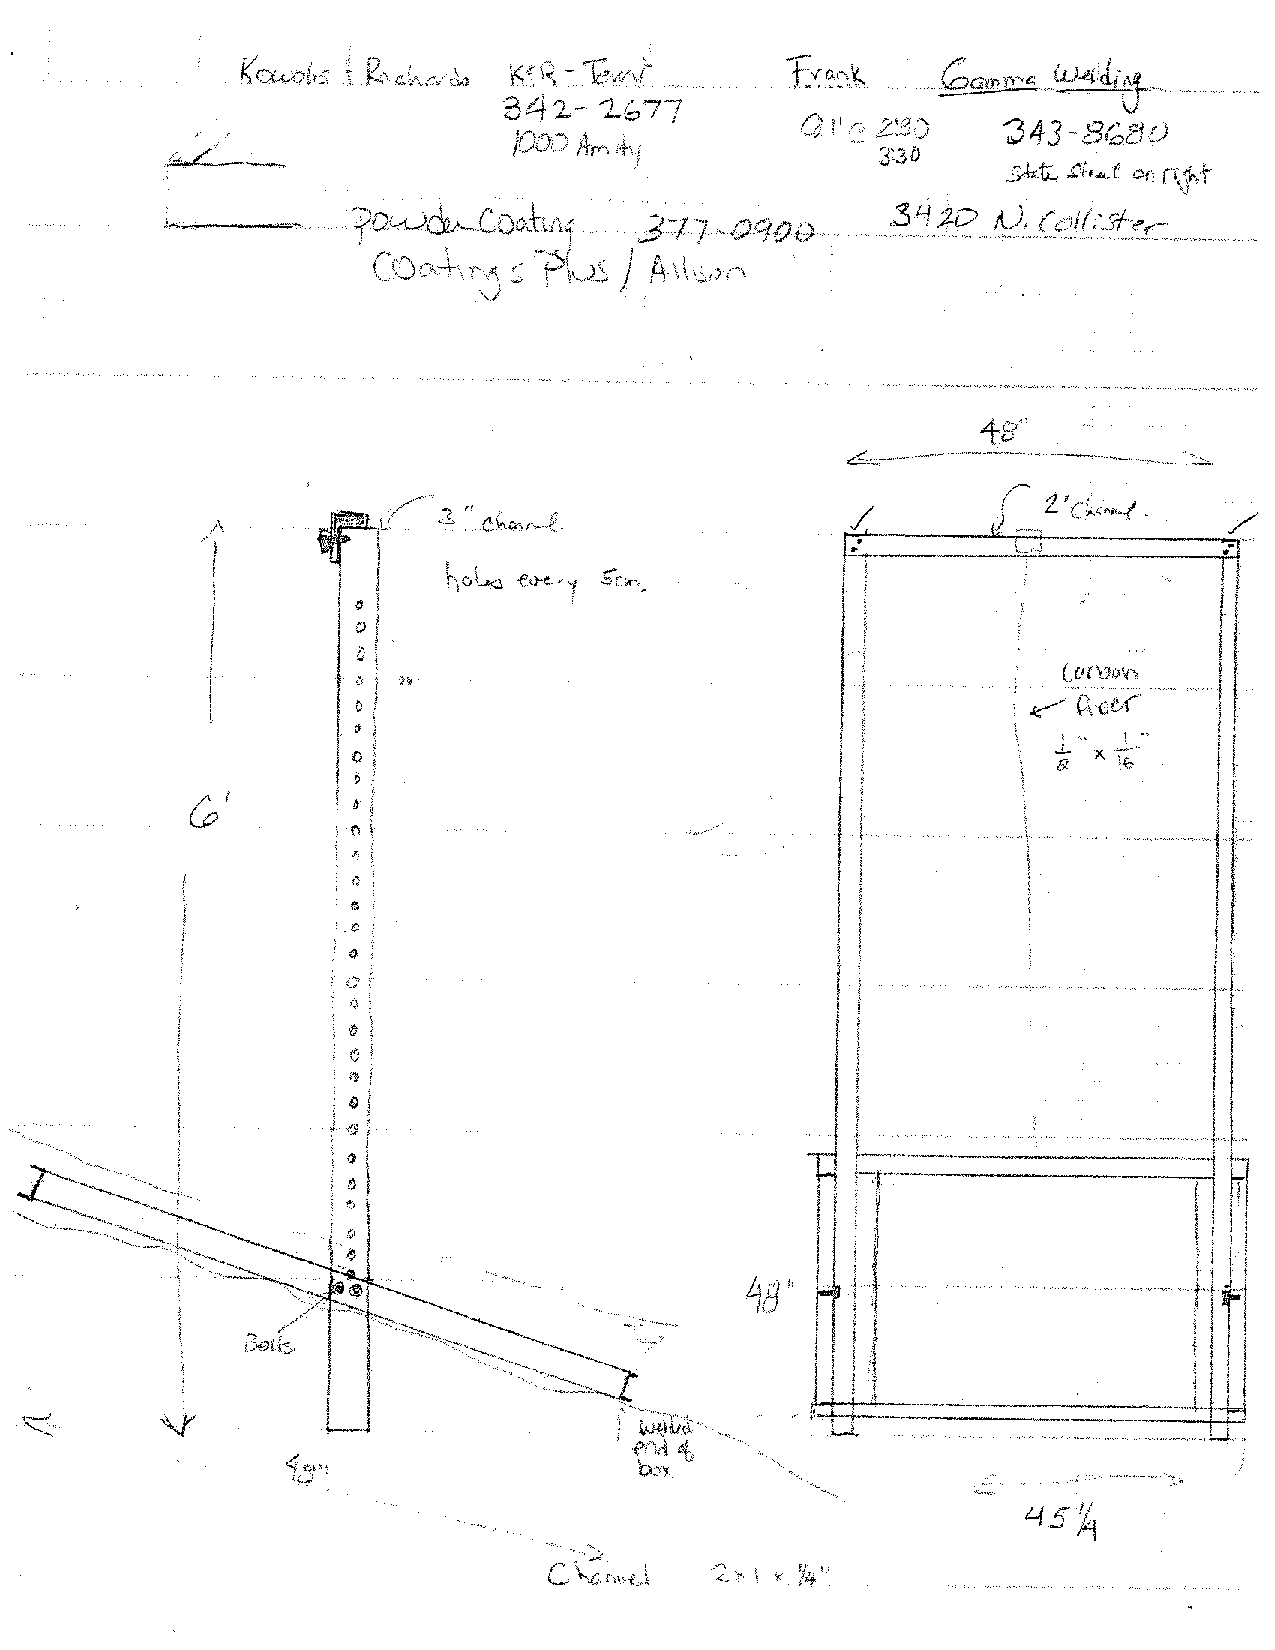
\includepdf[]{USFS_design/Luce_Black1.pdf}
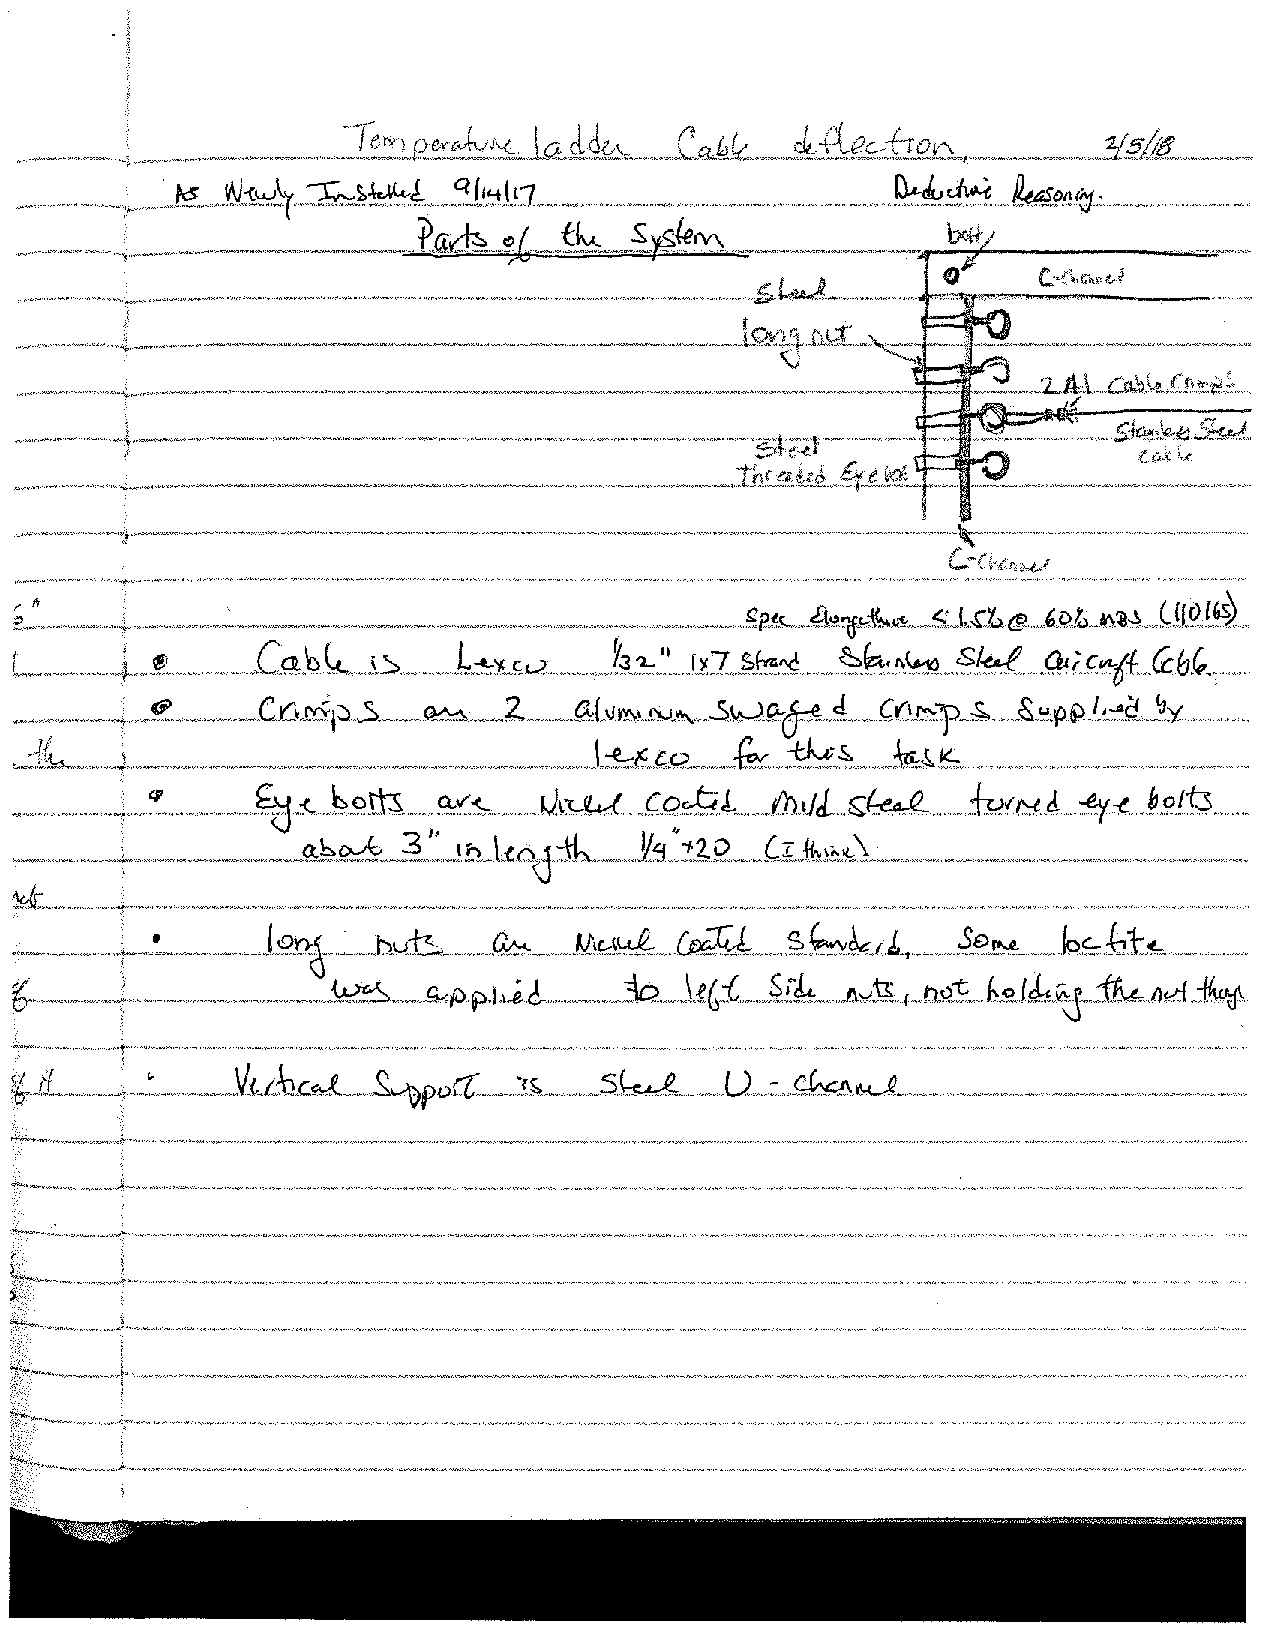
\includepdf[]{USFS_design/Luce_Black2.pdf}
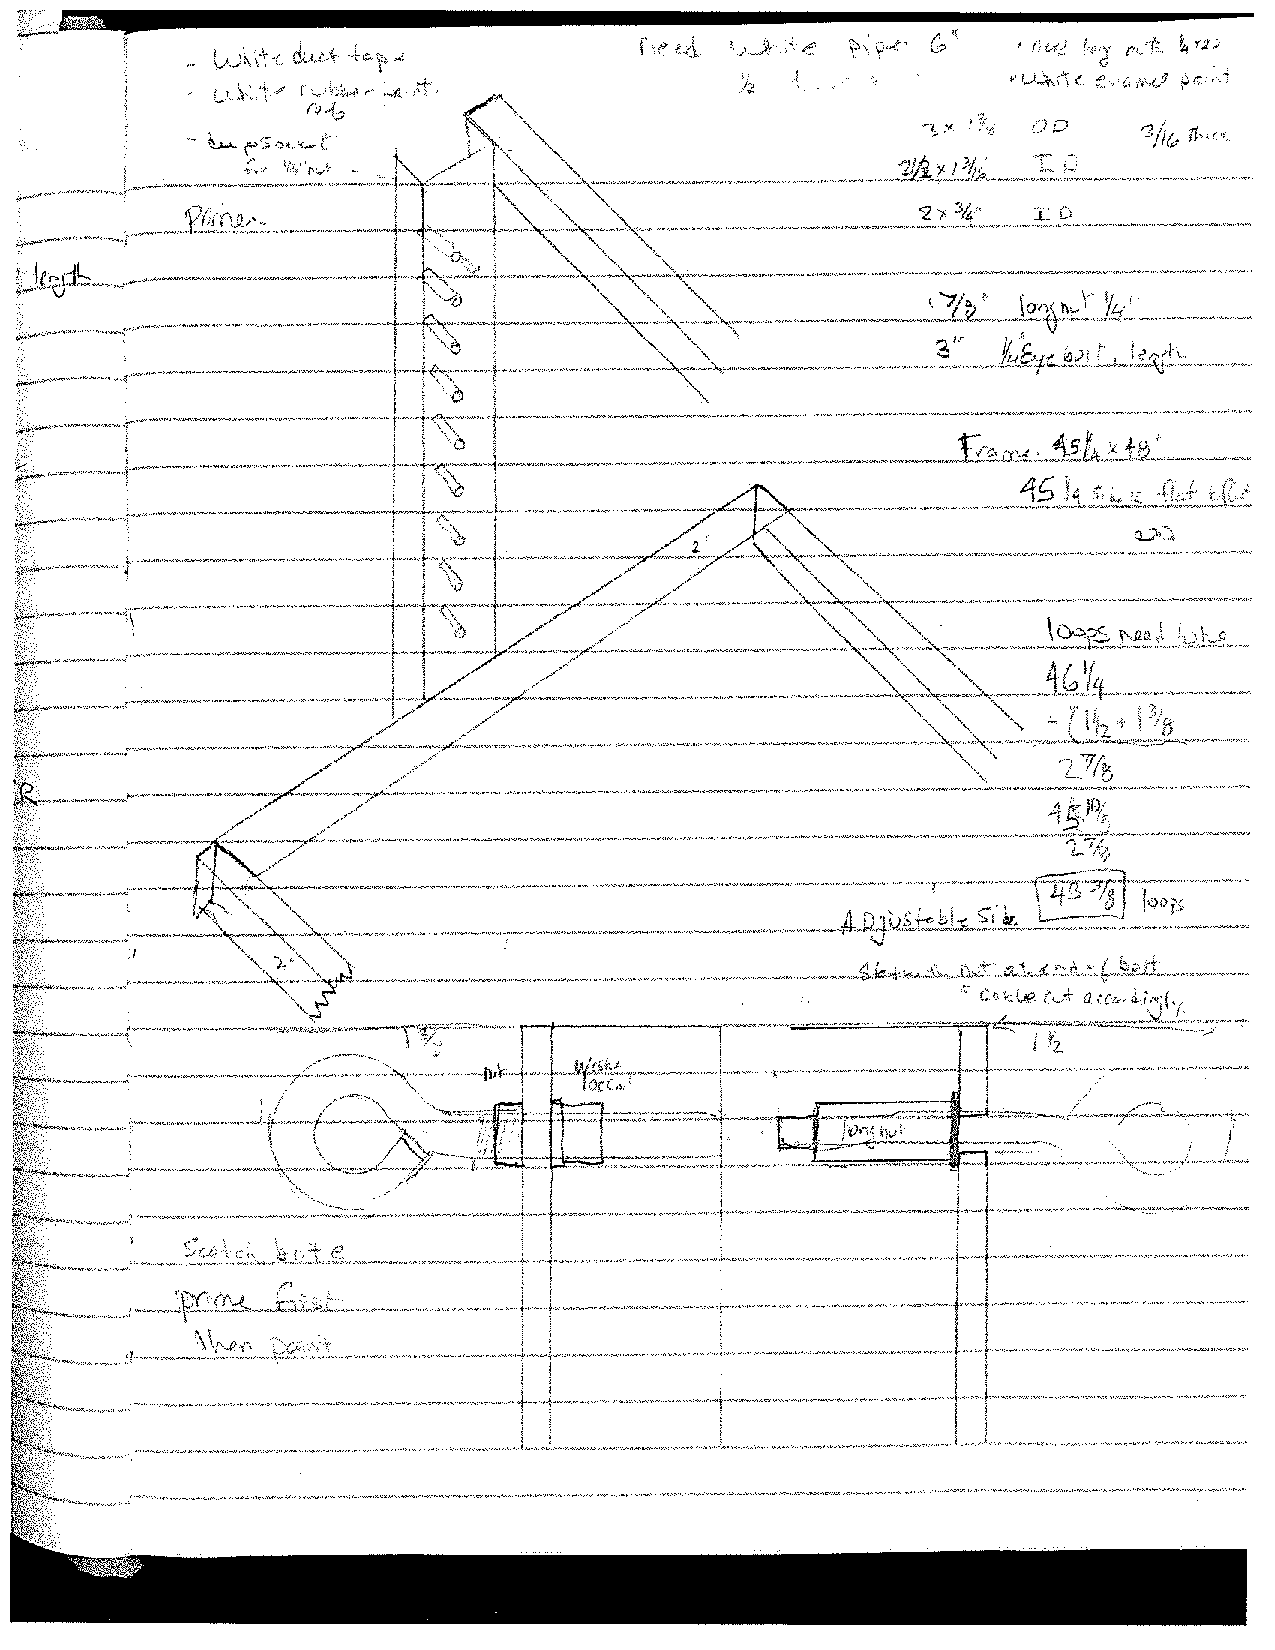
\includepdf[]{USFS_design/Luce_Black3.pdf}
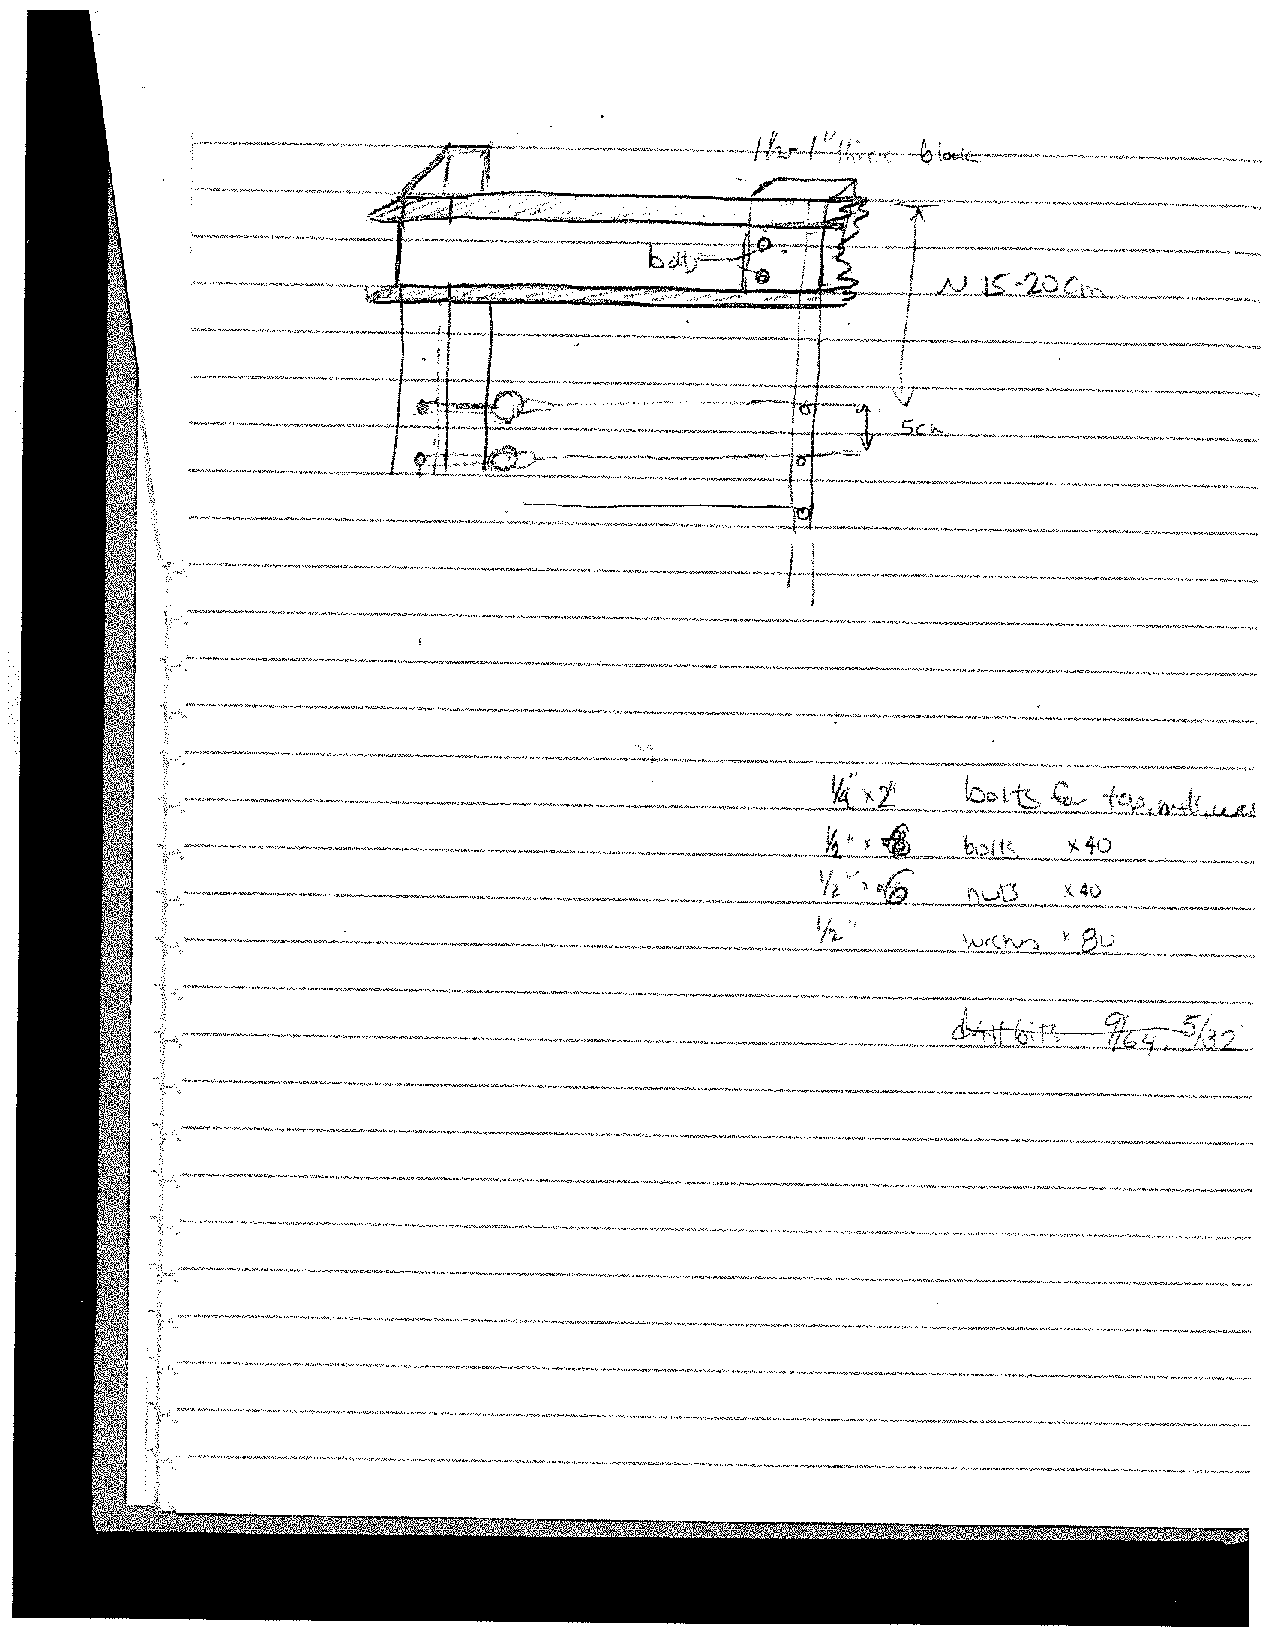
\includepdf[]{USFS_design/Luce_Black4.pdf}
\chapter{Data}
\section{Water Year 2019 Data}
\section{2020 Live Data}


